%Master File:lectures.tex

\lesson{Ensemble Methods}
\vspace{-1cm}
\begin{center}
  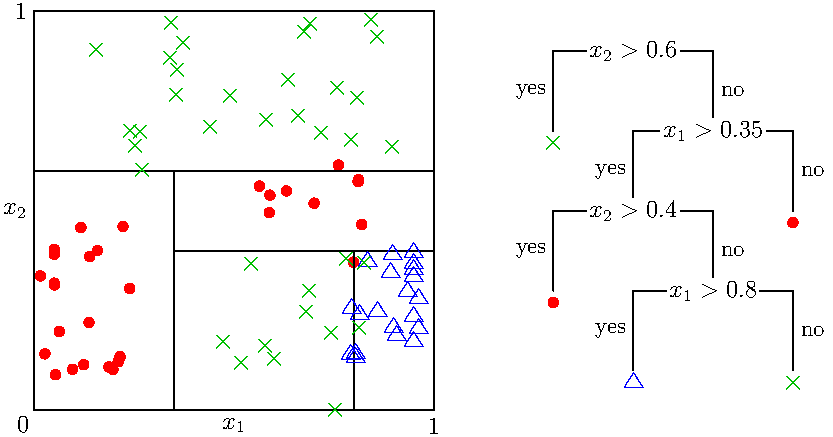
\includegraphics[height=12cm]{decisionTree-5}
\end{center}

\keywords{Decision Trees, Bagging, Boosting}


%%%%%%%%%%%%%%%%%%%%%%% Next Slide %%%%%%%%%%%%%%%%%%%%%%%
\renewcommand{\Outline}{%
\begin{slide}
\section[1]{Outline}

\begin{minipage}{8cm}\raggedright
  \begin{enumerate}
    \outlineitem{Decision Trees}{decisiontreees}
    \outlineitem{Bagging}{bagging}
    \outlineitem{Boosting}{boosting}
  \end{enumerate}
\end{minipage}\hfill
\begin{minipage}{15cm}
  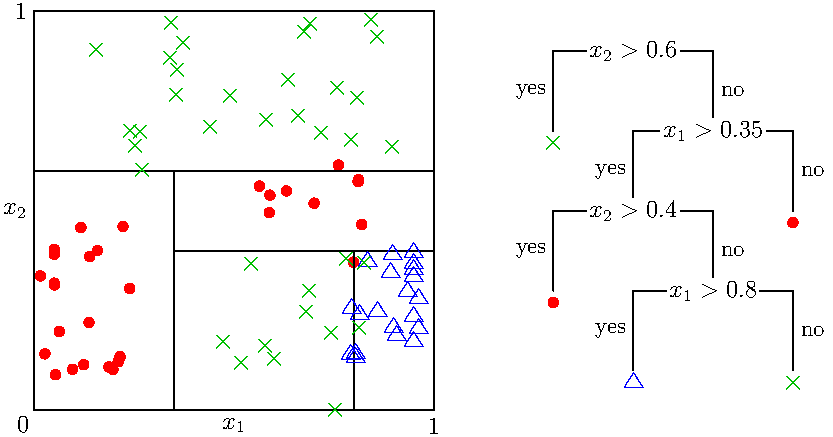
\includegraphics[width=15cm]{decisionTree-5}
\end{minipage}
\end{slide}
\addtocounter{outlineitem}{1}
}

\setcounter{outlineitem}{1}

%%%%%%%%%%%%%%%%%%%%%%% Next Slide %%%%%%%%%%%%%%%%%%%%%%%
\Outline %  Ensemsble Learning
\toptarget{firstoutline}
%%%%%%%%%%%%%%%%%%%%%%% Next Slide %%%%%%%%%%%%%%%%%%%%%%%

\begin{slide}
\section{Removing Variance By Averaging}

\begin{PauseHighLight}
  \begin{itemize}
  \item We can reduce the variance and hence improve our generalisation
    error by averaging over different learning machines\pause
  \item There are a number of different techniques for doing this that
    go by the name of \emph{ensemble methods} or \emph{ensemble
      learning}\pause
  \item This trick can be used with many different learning machines,
    but is clearly most practical for machine that can be trained
    quickly\pause
  \item (nevertheless, even for deep learning taking the average
    response of many machines is usually done to win competitions)\pauseb
  \end{itemize}
\end{PauseHighLight}

\end{slide}

%%%%%%%%%%%%%%%%%%%%%%% Next Slide %%%%%%%%%%%%%%%%%%%%%%%

\begin{slide}
\section{Ensembling of Decision Trees}

\begin{PauseHighLight}
  \begin{itemize}
  \item One set of algorithms where ensembling are common place are
    decision trees\pause
  \item These are particularly good for handling messy data
    \begin{itemize}
    \item categorical data\pause
    \item mixture of data types\pause
    \item missing data\pause
    \item large data sets\pause
    \item multiclass\pause
    \end{itemize}
  \item In many competitions ensembled trees, particularly
    \textit{random forests} and \textit{gradient boosting} beats all
    other techniques\pause
  \end{itemize}
\end{PauseHighLight}

\end{slide}

%%%%%%%%%%%%%%%%%%%%%%% Next Slide %%%%%%%%%%%%%%%%%%%%%%%

\begin{slide}
\section{Decision Trees}

\begin{PauseHighLight}
  \begin{itemize}
  \item Decision trees builds a binary tree to partition the data,
    $\mathcal{D}=\{(\bm{x}_i, y_i)|i=1,\ldots,m\}$, into the leaves of
    the tree\pause
  \item Each decision rule depends on a single feature\pause
  \item At each step the rule is chosen that maximise the
    ``\textit{purity}'' of the leaf nodes\pause
  \item Decisions can be made on numerical values or categories\pause
  \end{itemize}
\end{PauseHighLight}

\end{slide}

%%%%%%%%%%%%%%%%%%%%%%% Next Slide %%%%%%%%%%%%%%%%%%%%%%%

\begin{slide}
\section[-2]{Partitioning}

\begin{PauseHighLight}
  \begin{itemize}
  \item Consider a classification problems with examples $(\bm{x}, y)$
    belonging to some classes $y\in\mathcal{C}$\pause
  \item The data is partitioned by the tree into leaves
    \begin{center}
      \includegraphics[width=0.62\linewidth]{treePicture}\pause
    \end{center}
    \vspace*{-1.6em}

  \item The proportion of data points in leaf $\mathcal{L}$ belonging to
    class $c$ is
    \begin{align*}
      p_{c}(\mathcal{L}) = \frac{1}{|\mathcal{L}|}
      \sum_{(\bm{x},y)\in\mathcal{L}} \pred{y = c}
    \end{align*}
    where $\pred{y = c} = 1$ if $y=c$ and 0 otherwise\pause
  \end{itemize}
\end{PauseHighLight}

\end{slide}

%%%%%%%%%%%%%%%%%%%%%%% Next Slide %%%%%%%%%%%%%%%%%%%%%%%

\begin{slide}
\section{Leaf Purity}

\begin{PauseHighLight}
  \begin{itemize}
  \item Two different purity measures, $Q_m(\mathcal{L})$, for a leaf node
    $\mathcal{L}$ are commonly used\pause
    \begin{itemize}
    \item \emph{Gini index}
      \begin{rightImage}{gini}
        \begin{align*}
          Q^g_m(\mathcal{L}) = \sum_{c\in\mathcal{C}} p_{c}(\mathcal{L})\,
          \left(1-p_{c}(\mathcal{L})\right)\pause
        \end{align*}
      \end{rightImage}
    \item \emph{Cross-entropy}
      \begin{rightImage}{crossEnt}
        \begin{align*}
          Q^e_m(\mathcal{L}) = - \sum_{c\in\mathcal{C}} p_{c}(\mathcal{L})\,
          \logg{p_{c}(\mathcal{L})} \pause        
        \end{align*}
      \end{rightImage}
    \end{itemize}
  \end{itemize}
\end{PauseHighLight}

\end{slide}


%%%%%%%%%%%%%%%%%%%%%%% Next Slide %%%%%%%%%%%%%%%%%%%%%%%

\begin{slide}
\section[-1]{Building Decision Trees}

\pb\pause\pauselevel{=1}
\begin{center}
  \multipdf[width=\linewidth]{decisionTree}\pause
\end{center}

\end{slide}

%%%%%%%%%%%%%%%%%%%%%%% Next Slide %%%%%%%%%%%%%%%%%%%%%%%

\begin{slide}
\section{Observations}

\begin{PauseHighLight}
  \begin{itemize}
  \item Decision trees are very useful for exploring new data
    sets\pause---the tree shows what features are most
    important\pause
  \item Decision trees can also be used for regression problems\pause
    \begin{itemize}
    \item Approximate function by a series of steps\pause
    \item Reduce variance between data points assigned to leaf
      nodes\pause
    \end{itemize}
  \item CART is a classic implementation that builds
    \emph{C}lassification \emph{A}nd \emph{R}egression
    \emph{T}rees\pause
  \item Decision trees depend strongly on the early decisions and so
    vary a lot for slightly different data sets\pause---high variance\pauseb
  \end{itemize}
\end{PauseHighLight}

\end{slide}

%%%%%%%%%%%%%%%%%%%%%%% Next Slide %%%%%%%%%%%%%%%%%%%%%%%
\Outline %  Bagging
%%%%%%%%%%%%%%%%%%%%%%% Next Slide %%%%%%%%%%%%%%%%%%%%%%%


\begin{slide}
  \section[-2]{Error In The Means}
  \pb
  \begin{itemize}
  \item By taking the mean over many samples we can reduce out
    variance and thus improve our generalisation performance\pauseh
  \item To get a feel for this consider estimating the mean of a
    random variable $X$, from a number of samples ($n=5$ in the
    example below)\pauseh    
  \end{itemize}
    \begin{center}
      \multipdf[width=\linewidth]{standardError}\pause
    \end{center}
\end{slide}

%%%%%%%%%%%%%%%%%%%%%%% Next Slide %%%%%%%%%%%%%%%%%%%%%%%

\begin{slide}
\section[-2]{Mean and Variance}

\begin{PauseHighLight}\small
  \begin{itemize}
  \item The expected value of the mean, $\hat{\mu}_n$ of $n$ random
    \emph{independent} variables, $X_i$, is the expected value $\mu=\av{X_i}$
    \begin{align*}
      \av{\hat{\mu}_n}
      =\av{\frac{1}{n} \sum_{i=1}^n X_i } = \frac{1}{n} \sum_{i=1}^n
      \av{X_i} \pause = \frac{1}{n} \sum_{i=1}^n \mu = \mu\pause
    \end{align*}
  \item The variance is $\av{ (\hat{\mu}_n-\mu)^2 }$ or equivalently 
    \begin{align*}
      \frac{1}{n^2} \, \av{ \left(\sum_{i=1}^n (X_i -\mu)\right)^2}
      &=\frac{1}{n^2} \, \av{ \sum_{i=1}^n (X_i -\mu)^2
        + \sum_{i=1}^n\sum_{j=1\atop j\neq i}^n (X_i-\mu)\,(X_j-\mu)}\pause\\
      &= \frac{1}{n^2}\sum_{i=1}^n \left( \av{(X_i -\mu)^2}
        + \sum_{j=1\atop j\neq i}^n
      \av{X_i-\mu}\,\av{X_j-\mu} \right)\pause\\
      &=\frac{1}{n^2} \sum_{i=1}^n \sigma^2\pause = \frac{1}{n} \sigma^2
        \pause
    \end{align*}
  \end{itemize}
\end{PauseHighLight}


\end{slide}

%%%%%%%%%%%%%%%%%%%%%%% Next Slide %%%%%%%%%%%%%%%%%%%%%%%

\begin{slide}
\section[-2]{Bootstrap Aggregation (Bagging)}

\pb
\begin{itemize}
\item To reduce the variance in a learning machine (such as a decision
  tree) we can average over many machines\pauseh
\item To average many machines they must learn something different\pauseh
\item We only have one data set, but we can resample from the data set
  to make them look a bit different\pauseh---this is known a
  \emph{bootstrapping}\pauseh
\end{itemize}
\begin{center}
  \multipdf[width=\linewidth]{bootstrapping}\pause
\end{center}

\end{slide}

%%%%%%%%%%%%%%%%%%%%%%% Next Slide %%%%%%%%%%%%%%%%%%%%%%%

\begin{slide}
\section{Performance of Bagging}

\begin{PauseHighLight}
  \begin{itemize}
  \item For classification we get our different machines to vote\pause
  \item For regression we can average the prediction of different
    machines\pause
  \item Bagging improves the performance of decision trees\pause
  \item However, we can usually do better using Boosting\pause
  \item This is because our decision trees are correlated\pause
  \end{itemize}
\end{PauseHighLight}

\end{slide}


%%%%%%%%%%%%%%%%%%%%%%% Next Slide %%%%%%%%%%%%%%%%%%%%%%%

\begin{slide}
\section{Variance of Positive Correlated Variables}

\begin{PauseHighLight}
  \begin{itemize}
  \item If we calculate the variance of the mean of positively correlated
    variables with correlation $\rho$ we find
    \begin{align*}
      \frac{1}{n^2} \, \av{ \left(\sum_{i=1}^n X_i -\mu\right)^2}
      &= \rho\,\sigma^2 + \frac{1-\rho}{n} \sigma^2
    \end{align*}
  ($\rho = \av{(X_i-\mu)\,(X_j-\mu)}/\sigma^2$)\pause
  \item As $n\rightarrow\infty$ the second term vanishes, but we are left
    with the first term\pause
  \item If we want to do well we need our learning machines to be
    unbiased and decorrelated\pause
  \end{itemize}
\end{PauseHighLight}


\end{slide}


%%%%%%%%%%%%%%%%%%%%%%%xt Slide %%%%%%%%%%%%%%%%%%%%%%%

\begin{slide}
\section{Random Forest}

\begin{PauseHighLight}
  \begin{itemize}
  \item In random forests we average much less correlated trees\pause
  \item We do this for each tree we choose a subset of $p'\ll p$ of the
    features on which to split the tree\pause
  \item Typically $p'$ can range from 1 to $\sqrt{p}$\pause
  \item The trees aren't that good, but are very decorrelated\pause
  \item By averaging over a huge number of trees (order of 1000) we
    typically get good results\pause
  \item Random Forest won (wins?) many competitions\pause
  \end{itemize}
\end{PauseHighLight}

\end{slide}

%%%%%%%%%%%%%%%%%%%%%%% Next Slide %%%%%%%%%%%%%%%%%%%%%%%
\Outline %  Boosting
%%%%%%%%%%%%%%%%%%%%%%% Next Slide %%%%%%%%%%%%%%%%%%%%%%%

\begin{slide}
\section{Boosting}

\begin{PauseHighLight}
  \begin{itemize}
  \item In boosting we make a \emph{strong learner} by using a weighted
    sum of \emph{weak learners}
    \begin{align*}
      C_n(\bm{x}) = \sum_{i=1}^n \alpha_i \, \hat{h}_i(\bm{x})\pause
    \end{align*}
  \item Weak learners, $\hat{h}_i(\bm{x})$, are learning machine that do a
    little better than chance\pause
  \item The trick is to choose the weights, $\alpha_i$\pause
  \item Because the weak learners do little better than chance we
    (miraculously) \textbf{don't} overfit\pause{} that much\pauseb
  \end{itemize}
\end{PauseHighLight}

\end{slide}

%%%%%%%%%%%%%%%%%%%%%%% Next Slide %%%%%%%%%%%%%%%%%%%%%%%

\begin{slide}
\section{Shallow Trees}

\begin{PauseHighLight}
  \begin{itemize}
  \item One of the most effective type of weak learner are very shallow
    trees\pause
  \item Sometimes we just use one variable (the stump)\pause
  \item There are different algorithms for choosing the weights
    \begin{itemize}
    \item adaboost\pause---a classic algorithm for binary problems\pauseb
    \item gradient boosting\pause---used for regression, trains a
      classifier on the residual errors\pauseb
    \end{itemize}
  \end{itemize}
\end{PauseHighLight}

\end{slide}
%%%%%%%%%%%%%%%%%%%%%%% Next Slide %%%%%%%%%%%%%%%%%%%%%%%

\begin{slide}
\section{Boosting a Binary Classifier}

\begin{PauseHighLight}
  \begin{itemize}
  \item Suppose we have a binary classification task with data
    $\mathcal{D} = \{(\bm{x}^\mu, y^\mu)| \mu=1,\,2,\,\ldots,\,
    m\}$ with $y^\mu\in\{-1,1\}$\pause
  \item Our $i^{th}$ weak learner provides a prediction
    $\hat{h}_i(\bm{x}^\mu)\in \{-1,1\}$\pause
  \item We ask, can we find a linear combination
    \begin{align*}
      C_n(\bm{x}) = \alpha_1 \, \hat{h}_1(\bm{x}) + \alpha_2 \,
      \hat{h}_2(\bm{x}) + \cdots +  \alpha_n \, \hat{h}_n(\bm{x})
    \end{align*}
  \item So that $\mathrm{sgn}\!\left(\strut C_n(\bm{x}) \right)$ is a
    strong learner?\pause
  \end{itemize}
\end{PauseHighLight}

\end{slide}

%%%%%%%%%%%%%%%%%%%%%%% Next Slide %%%%%%%%%%%%%%%%%%%%%%%

\begin{slide}
\section[-2]{AdaBoost}

\begin{PauseHighLight}
  \begin{itemize}
  \item AdaBoost is a classic solution to this problem\pause
  \item It assigns an ``loss function''\\
    \begin{minipage}{0.48\linewidth}
      \begin{align*}
        L_n = \sum_{\mu=1}^m \e{-y^\mu C_n(\bm{x}^\mu)}\pause
      \end{align*}
    \end{minipage}\hfil
    \begin{minipage}{0.48\linewidth}
      \includegraphics[width=0.9\linewidth]{adaboostError}
    \end{minipage}
  \item This punishes examples where there is an errors more than
    correct classifications\pause
  \end{itemize}
\end{PauseHighLight}

\end{slide}

%%%%%%%%%%%%%%%%%%%%%%% Next Slide %%%%%%%%%%%%%%%%%%%%%%%

\begin{slide}
\section[-2]{Iterative Learning}

\begin{PauseHighLight}
  \begin{itemize}
  \item We build up a strong learner iteratively (greedily)
    \begin{align*}
       C_n(\bm{x}) =  C_{n-1}(\bm{x}) + \alpha_n \, \hat{h}_n(\bm{x})\pause
    \end{align*}
  \item Defining $w_1^\mu=1$ and $w_n^\mu = \e{-y^\mu C_{n-1}(\bm{x}^\mu)}$
    then
    \begin{align*}
      L_n(\alpha_n) &= \sum_{\mu=1}^m \e{-y^\mu C_n(\bm{x}^\mu)} \pause
                    = \sum_{\mu=1}^m \e{-y^\mu (C_{n-1}(\bm{x}^{\mu}) +
      \alpha_n \, \hat{h}_n(\bm{x}^\mu))}\pause \\
                    &=
      \sum_{\mu=1}^m w_n^\mu \, \e{-\alpha_n\, y^\mu\, \hat{h}_n(\bm{x}^\mu)}
                      \pause
      =  \sum_{\mu:y^\mu\neq \hat{h}_n(\bm{x}^\mu)}\hspace{-1.5em}  w_n^\mu\,
      \e{\alpha_n} \;\; + \hspace{-1em}
      \sum_{\mu:y^\mu= \hat{h}_n(\bm{x}^\mu)} \hspace{-1.5em} w_n^\mu\, \e{-\alpha_n}\pause
      \\
      &= \e{-\alpha_n} \sum_{\mu=1}^m w_n^\mu  +
        (\e{\alpha_n}-\e{-\alpha_n})\hspace{-1.5em} 
        \sum_{\mu:y^\mu\neq \hat{h}_n(\bm{x}^\mu)} w_n^\mu\pause
    \end{align*}
   \end{itemize}
\end{PauseHighLight}

\end{slide}


%%%%%%%%%%%%%%%%%%%%%%% Next Slide %%%%%%%%%%%%%%%%%%%%%%%

\begin{slide}
\section[-2]{Choosing a Weak Classifier}

\begin{PauseHighLight}
  \begin{itemize}
  \item To minimise the error
    \begin{align*}
       L_n(\alpha_n)  &= \e{-\alpha_n} \sum_{\mu=1}^m w_n^\mu +
        (\e{\alpha_n}-\e{-\alpha_n})\hspace{-1.5em} 
        \sum_{\mu:y^\mu\neq \hat{h}_n(\bm{x}^\mu)} w_n^\mu\pause
    \end{align*}
  \item We choose the weak learner with the lowest value of
    \begin{rightImage}{adaboostErrorPrev}
      \begin{align*}
        \sum_{\mu:y^\mu\neq \hat{h}_n(\bm{x}^\mu)}\!\!\! w_n^\mu
        =  \sum_{\mu:y^\mu\neq \hat{h}_n(\bm{x}^\mu)} \!\!\! \e{-y^\mu\,C_{n-1}(\bm{x}^\mu)}
        \pause
      \end{align*}  
    \end{rightImage}
  \item That is, it misclassifies only where the other learners classify
    well\pause 
  \end{itemize}
\end{PauseHighLight}

\end{slide}

%%%%%%%%%%%%%%%%%%%%%%% Next Slide %%%%%%%%%%%%%%%%%%%%%%%

\begin{slide}
\section{Choosing Weights}

\begin{PauseHighLight}
  \begin{itemize}
  \item We now choose the weight $\alpha_n$ to minimise the error $L_n(\alpha_n)$
    \begin{align*}
      \pd{L_n(\alpha_n)}{\alpha_n} = 
       \e{\alpha_n} \hspace{-1em} \sum_{\mu:y^\mu\neq
      \hat{h}_n(\bm{x}^\mu)} \hspace{-1.5em}  w_n^\mu\, \;- 
      \e{-\alpha_n} \hspace{-1em} \sum_{\mu:y^\mu= \hat{h}_n(\bm{x}^\mu)}
      \hspace{-1.5em} w_n^\mu =0\pause
    \end{align*}
  \item That is
    \begin{align*}
      \e{2\,\alpha_n} &= \frac{\displaystyle \sum_{\mu:y^\mu=
      \hat{h}_n(\bm{x}^\mu)} \hspace{-1.5em} w_n^\mu}{\displaystyle
                        \sum_{\mu:y^\mu\neq \hat{h}_n(\bm{x}^\mu)} \hspace{-1.5em} w_n^\mu}\pause
                        & \text{or}& &
     \alpha_n &= \frac{1}{2} \logg{\frac{\displaystyle \sum_{\mu:y^\mu=
      \hat{h}_n(\bm{x}^\mu)} \hspace{-1.5em} w_n^\mu}{\displaystyle
                \sum_{\mu:y^\mu\neq \hat{h}_n(\bm{x}^\mu)}\hspace{-1.5em} w_n^\mu}}\pause
    \end{align*}
  \end{itemize}
\end{PauseHighLight}

\end{slide}

%%%%%%%%%%%%%%%%%%%%%%% Next Slide %%%%%%%%%%%%%%%%%%%%%%%

\begin{slide}
\section[-2]{Algorithm}

\begin{PauseHighLight}
  \small
  \begin{enumerate}
  \item Start with a set of weak learners $\mathcal{W}$\pause
  \item Associate a weight, $w_n^\mu$, with every data point
    $(\bm{x}^\mu, y^\mu)$, $\mu=1,2,\ldots,m$\pause
  \item Initially $w_0^\mu=1$\pause{} (large weight, $w_n^\mu$, means
    $(\bm{x}^\mu, y^\mu)$ is poorly classified)\pauseb
  \item Choose the weak learning, $\hat{h}_n(\bm{x})\in\mathcal{W}$, that minimises
    $\sum\limits_{\mu:y^\mu\neq \hat{h}_n(\bm{x}^\mu)}\!\!\!
    w_n^\mu$\pause
  \item Update predictor $C_n(\bm{x}) = C_{n-1}(\bm{x}) + \alpha_n \,
    \hat{h}_n(\bm{x})$ where $\alpha_n=  \frac{1}{2} \logg{\frac{\sum\limits_{\mu:y^\mu=
      \hat{h}_n(\bm{x}^\mu)}  w_n^\mu}{
                \sum\limits_{\mu:y^\mu\neq \hat{h}_n(\bm{x}^\mu)}\ w_n^\mu}}$\pause
  \item Update $w_{n+1}^\mu = w_{n}^\mu\, \e{-y^\mu\, \alpha_n \, \hat{h}_n(\bm{x}^\mu)}$\pause
  \item Go to 4\pause
  \end{enumerate}
\end{PauseHighLight}

\end{slide}


%%%%%%%%%%%%%%%%%%%%%%% Next Slide %%%%%%%%%%%%%%%%%%%%%%%

\begin{slide}
\section{Performance}

\begin{PauseHighLight}
  \begin{itemize}
  \item Adaboost works well with weak learners, usually out-performing
    bagging\pause
  \item It doesn't work well with strong learners (tends to
    over-fit)\pause
  \item It is limited to binary classification (there are
    generalisation, but they are difficult to get to work)\pause
  \item It has fallen from fashion\pause
  \item In contrast \emph{gradient boosting} used for regression is
    very popular\pause
  \end{itemize}
\end{PauseHighLight}

\end{slide}

%%%%%%%%%%%%%%%%%%%%%%% Next Slide %%%%%%%%%%%%%%%%%%%%%%%

\begin{slide}
\section{Gradient Boosting}

\begin{PauseHighLight}
  \begin{itemize}
  \item In gradient boosting we again build a strong learner as a linear
    combination of weak learners
    \begin{align*}
      C_n(\bm{x}) = C_{n-1}(\bm{x}) + \hat{h}_n(\bm{x})\pause
    \end{align*}
  \item At each step $\hat{h}_n(\bm{x})$ is trained to predict the
    residual error, $\Delta_{n-1} = y-C_{n-1}(\bm{x})$, (i.e. the target minus
    the current prediction)\pause
  \item (This difference looks a bit like a gradient hence the rather
    confusing name)\pause
  \item Gradient boosting also mainly used with regression decision trees\pause
  \end{itemize}
\end{PauseHighLight}

\end{slide}

%%%%%%%%%%%%%%%%%%%%%%% Next Slide %%%%%%%%%%%%%%%%%%%%%%%

\begin{slide}
\section[-1]{}

\begin{center}
  \includegraphics[width=0.7\linewidth]{gb1}
\end{center}
\end{slide}

%%%%%%%%%%%%%%%%%%%%%%% Next Slide %%%%%%%%%%%%%%%%%%%%%%%

\begin{slide}
\section{Keep On Going}
\pb
\begin{itemize}
\item We can keep on going
\end{itemize}
\begin{center}
  \includegraphics[width=\linewidth]{gb2}\pauseh
\end{center}
\begin{itemize}
\item But we will over-fit eventually\pause
\end{itemize}
\end{slide}

%%%%%%%%%%%%%%%%%%%%%%% Next Slide %%%%%%%%%%%%%%%%%%%%%%%

\begin{slide}
\section{Early Stopping}

\pb
\begin{itemize}
\item Like many algorithms we often get better results by early
  stopping\pauseh
\end{itemize}
\begin{center}
  \includegraphics[width=\linewidth]{gb3}
\end{center}
\begin{itemize}
\item Use cross-validation against a validation set to decide when to
  stop\pauseh
\end{itemize}

\end{slide}

%%%%%%%%%%%%%%%%%%%%%%% Next Slide %%%%%%%%%%%%%%%%%%%%%%%

\begin{slide}
\section[-2]{XGBoost}

\begin{PauseHighLight}
  \begin{itemize}
  \item XGBoost is an implementation of gradient boosting that won the
    Higg's Boson challenge and regularly wins Kaggle competitions\pause
  \item XGBoost stands for eXtreme Gradient Boosting\pause
  \item It was much faster than most gradient boosting algorithms and
    scales to billions of training data points---although GBM is often
    better\pause
  \item It uses a cleverly chosen regularisation term to favour simple
    trees\pause
  \item Finds a clever way to approximately minimise error plus
    regulariser very fast\pause
  \item Rather a bodge of optimisation hacks\pauseb
  \end{itemize}
\end{PauseHighLight}


\end{slide}

%%%%%%%%%%%%%%%%%%%%%%% Next Slide %%%%%%%%%%%%%%%%%%%%%%%

\begin{slide}
\section{Conclusion}

\begin{PauseHighLight}
  \begin{itemize}
  \item Ensemble methods have proved themselves to be very
    powerful\pause
  \item Tend to work best with very simple models (true of random forest
    and boosting)\pause---seems to reduce over-fitting\pauseb
  \item XGBoost or GBM are currently the best methods for tabular data
    (particular for large training sets)\pause---probably\pauseb
  \item For images, signal and speech deep learning can give very
    significant advantage\pause
  \item Probabilistic models can be better if you have a good model\pause
  \end{itemize}
\end{PauseHighLight}

\end{slide}


%%% Local Variables:
%%% TeX-master: "lectures"
%%% End:
